\documentclass{standalone}
\usepackage{tikz}
\usepackage{ctex,siunitx}
\setCJKmainfont{Noto Serif CJK SC}
\usepackage{tkz-euclide}
\usepackage{amsmath}
\usetikzlibrary{patterns, calc,3d}
\usetikzlibrary {decorations.pathmorphing,decorations.pathreplacing,decorations.shapes}
\tikzset{label style/.append style={font=\small}}
\begin{document}
\small
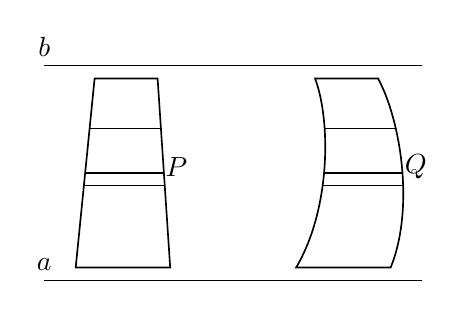
\begin{tikzpicture}[>=latex,scale=0.8]
  \draw(0,-0.2)node[above]{$a$}--(6,-0.2)(0,3.2)node[above]{$b$}--(6,3.2);
  \draw[semithick](0.5,0)--(0.8,3)--(1.8,3)--(2,0)--cycle;
  \draw(0.63,1.3)--++(1.2833,0)(0.65,1.5)--++(1.25,0)(0.72,2.2)--++(1.1333,0);
  \draw[semithick](4,0)..controls(4.5466,0.9289)and(4.5533,2.3185)..(4.3,3)--(5.3,3)..controls(5.6665,2.3185)and(5.8786,0.9289)..(5.5,0)--cycle;
  \draw(4.4201,1.3)--++(1.2833,0)(4.4425,1.5)--++(1.25,0)(4.4521,2.2)--++(1.1333,0);
  \node at (2.1,1.6){$P$};
  \node at (5.9,1.6){$Q$};
\end{tikzpicture}
\end{document}